\let\negmedspace\undefined
\let\negthickspace\undefined
\documentclass[journal]{IEEEtran}
\usepackage[a5paper, margin=10mm, onecolumn]{geometry}
\usepackage{lmodern} % Ensure lmodern is loaded for pdflatex
\usepackage{tfrupee} % Include tfrupee package

\setlength{\headheight}{1cm} % Set the height of the header box
\setlength{\headsep}{0mm}  % Set the distance between the header box and the top of the text

\usepackage{csquotes}
\usepackage{gvv-book}
\usepackage{gvv}
\usepackage{circuitikz}
\usepackage{cite}
\usepackage{amsmath,amssymb,amsfonts,amsthm}
\usepackage{algorithmic}
\usepackage{graphicx}
\usepackage{textcomp}
\usepackage{xcolor}
\usepackage{txfonts}
\usepackage{listings}
\usepackage{enumitem}
\usepackage{mathtools}
\usepackage{gensymb}
\usepackage{comment}
\usepackage[breaklinks=true]{hyperref}
\usepackage{tkz-euclide} 
\usepackage{listings}
% \usepackage{gvv}                                        
\def\inputGnumericTable{}                                 
\usepackage[latin1]{inputenc}                                
\usepackage{color}                                            
\usepackage{array}                                            
\usepackage{longtable}                                       
\usepackage{calc}                                             
\usepackage{multirow}                                         
\usepackage{hhline}                                           
\usepackage{ifthen}                                           
\usepackage{lscape}
\usepackage{caption}
\usepackage{tikz}
\usetikzlibrary{patterns}
\begin{document}

\bibliographystyle{IEEEtran}



\title{GATE 2020 CIVIL ENGINEERING}
\author{EE25BTECH11013 - Bhargav}
\maketitle
% \maketitle
% \newpage
% \bigskip
{\let\newpage\relax\maketitle}

\renewcommand{\thefigure}{\theenumi}
\renewcommand{\thetable}{\theenumi}
\setlength{\intextsep}{10pt} % Space between text and floats

\section*{GA -- General Aptitude}

\noindent \textbf{Q1 -- Q5 carry one mark each.}

\begin{enumerate}
\item It is a common criticism that most of the academicians live in their\underline{\hspace{2cm}}, so, they are not aware of the real life challenges. \hfill \brak{GATE \ CE \ 2020}
    
\begin{enumerate}
\item homes  
\item ivory towers  
\item glass palaces  
\item big flats
\end{enumerate}

\item His hunger for reading is insatiable. He reads indiscriminately. He is most certainly a/an \underline{\hspace{2cm}} reader. \hfill \brak{GATE \ CE \ 2020}

\begin{enumerate}
\item all-round  
\item precocious  
\item voracious  
\item wise
\end{enumerate}

\item Select the word that fits the analogy:

\begin{center}
    Fuse : Fusion :: Use : \underline{\hspace{2cm}}
\end{center} 
\hfill \brak{GATE \ CE \ 2020}

\begin{enumerate}
\begin{multicols}{4}
\item Usage  
\item User  
\item Uses  
\item Usion    
\end{multicols}

\end{enumerate}

\item If 0, 1, 2, \ldots, 7, 8, 9 are coded as O, P, Q, \ldots, V, W, X, then 45 will be coded as \underline{\hspace{2cm}}. \hfill \brak{GATE \ CE \ 2020}

\begin{enumerate}
\begin{multicols}{4}
\item TS  
\item ST  
\item SS  
\item SU    
\end{multicols}

\end{enumerate}

\item The sum of two positive numbers is 100. After subtracting 5 from each number, the product of the resulting numbers is 0. One of the original numbers is \underline{\hspace{2cm}}. \hfill \brak{GATE \ CE \ 2020}

\begin{enumerate}
\begin{multicols}{4}
\item $80$  
\item $85$  
\item $90$ 
\item $95$
\end{multicols}

\end{enumerate}

\noindent \textbf{Q6 -- Q10 carry two marks each.}

\item The American psychologist Howard Gardner expounds that human intelligence can be sub-categorised into multiple kinds, in such a way that individuals differ with respect to their relative competence in each kind. Based on this theory, modern educationists insist on prescribing multi-dimensional curriculum and evaluation parameters that enable development and assessment of multiple intelligences.\\[0.3cm]
Which of the following statements can be inferred from the given text? \hfill \brak{GATE \ CE \ 2020}

\begin{enumerate}
\item Howard Gardner insists that the teaching curriculum and evaluation needs to be multi-dimensional.  
\item Howard Gardner wants to develop and assess the theory of multiple intelligences.  
\item Modern educationists want to develop and assess the theory of multiple intelligences.  
\item Modern educationists insist that the teaching curriculum and evaluation needs to be multi-dimensional.  
\end{enumerate}

\item Five friends P, Q, R, S and T went camping. At night, they had to sleep in a row inside the tent. P, Q and T refused to sleep next to R since he snored loudly. P and S wanted to avoid Q as he usually hugged people in sleep.\\[0.2cm]
Assuming everyone was satisfied with the sleeping arrangements, what is the order in which they slept? \hfill \brak{GATE \ CE \ 2020}

\begin{enumerate}
\item RSPTQ  
\item SPRTQ  
\item QRSPT  
\item QTSPR  
\end{enumerate}

\item Insert seven numbers between 2 and 34, such that the resulting sequence including 2 and 34 is an arithmetic progression. The sum of these inserted seven numbers is\underline{\hspace{1cm}}. \hfill \brak{GATE \ CE \ 2020}

\begin{enumerate}
\begin{multicols}{4}
\item 120 
\item 124  
\item 126  
\item 130      
\end{multicols}

\end{enumerate}

\item The unit's place in $26591749^{1101016}$ is\underline{\hspace{1cm}}. \hfill \brak{GATE \ CE \ 2020}

\begin{enumerate}
\begin{multicols}{4}
\item $1$  
\item $3$  
\item $6$  
\item $9$ 
\end{multicols} 
\end{enumerate}

\item The total expenditure of a family, on different activities in a month, is shown in the pie -- chart. The extra money spent on education as compared to transport \brak{in percent} is\underline{\hspace{1cm}}. \hfill \brak{GATE \ CE \ 2020}

\begin{figure}[H]
    \centering
    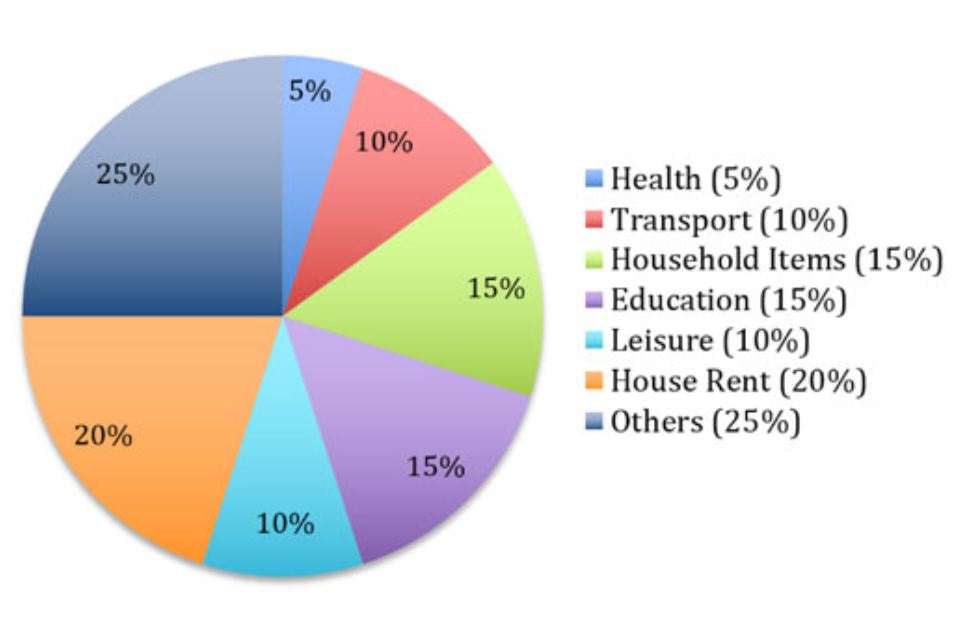
\includegraphics[width=0.3\columnwidth]{figs/Q10.png} 
    \caption{}
    \label{fig:placeholder}
\end{figure}

\begin{enumerate}
\begin{multicols}{4}
\item $5$  
\item $33.3$  
\item $50$  
\item $100$  
\end{multicols}
\end{enumerate}


\section*{CE -- CIVIL ENGINEERING}
\noindent \textbf{Q11 -- Q35 carry one mark each.}



\item In the following partial differential equation, $\theta$ is a function of $t$ and $z$, and $D$ and $K$ are functions of $\theta$:
\begin{align}
D(\theta)\,\frac{\partial^2 \theta}{\partial z^2} + \frac{\partial K(\theta)}{\partial z} - \frac{\partial \theta}{\partial t} = 0
\end{align}
The above equation is  \hfill \brak{GATE \ CE \ 2020}

\begin{enumerate}
\item a second order linear equation  
\item a second degree linear equation  
\item a second order non-linear equation  
\item a second degree non-linear equation  
\end{enumerate}

\item The value of 
\begin{align}
\displaystyle \lim_{x \to \infty} \frac{x^2 - 5x + 4}{4x^2 + 2x}
\end{align} is   \hfill \brak{GATE \ CE \ 2020}

\begin{enumerate}
\begin{multicols}{4}
\item $0$  
\item $\frac{1}{4}$  
\item $\frac{1}{2}$  
\item $1$  
\end{multicols}

\end{enumerate}

\item The true value of $\ln(2)$ is $0.69$. If the value of $\ln(2)$ is obtained by linear interpolation between $\ln(1)$ and $\ln(6)$, the percentage of absolute error \emph{(round off to the nearest integer)}, is  \hfill \brak{GATE \ CE \ 2020}

\begin{enumerate}
\begin{multicols}{4}
\item $35$  
\item $48$  
\item $69$  
\item $84$  
\end{multicols}

\end{enumerate}

\item The area of an ellipse represented by an equation 
\begin{align}
\displaystyle \frac{x^2}{a^2} + \frac{y^2}{b^2} = 1 
\end{align} is \hfill \brak{GATE \ CE \ 2020}

\begin{enumerate}
\begin{multicols}{4}
\item $\frac{\pi a b}{4}$  
\item $\frac{\pi a b}{2}$  
\item $\pi a b$  
\item $\frac{4 \pi a b}{3}$ 
\end{multicols}
 
\end{enumerate}

\item Consider the planar truss . Neglecting self-weight of the members, the number of zero-force members in the truss under the action of the load $P$ is \hfill \brak{GATE \ CE \ 2020}

\begin{figure}[H]
    \centering
    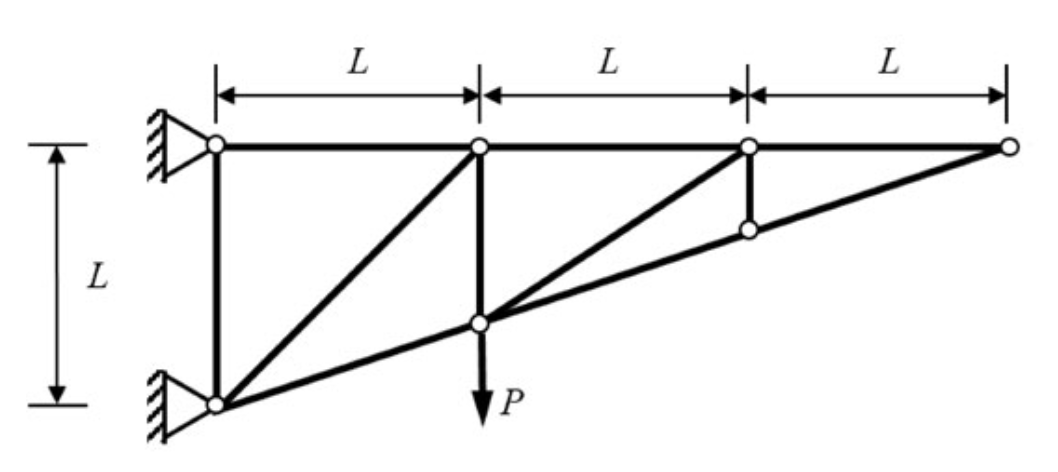
\includegraphics[width=0.3\columnwidth]{figs/Q15.png} 
    \caption{}
    \label{fig:placeholder}
\end{figure}

\begin{enumerate}
\begin{multicols}{4}
\item $6$  
\item $7$  
\item $8$  
\item $9$      
\end{multicols}

\end{enumerate}


\item A reinforcing steel bar, partially embedded in concrete, is subjected to a tensile force $P$. The figure that appropriately represents the distribution of the magnitude of bond stress \brak{represented \ as \ hatched \ region}, along the embedded length of the bar, is  \hfill \brak{GATE \ CE \ 2020}

\begin{enumerate}

\item 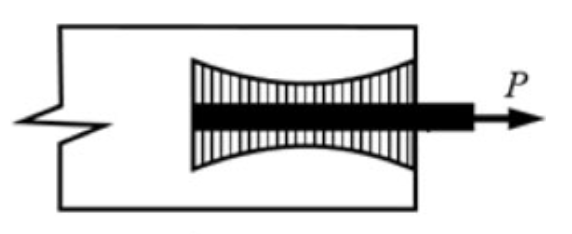
\includegraphics[width=0.3\columnwidth]{figs/Q16a.png}
\item 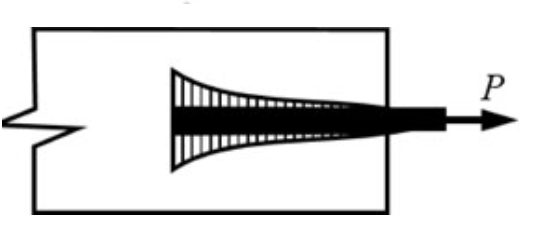
\includegraphics[width=0.3\columnwidth]{figs/Q16b.png}  
\item 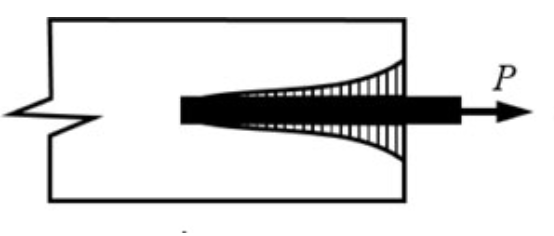
\includegraphics[width=0.3\columnwidth]{figs/Q16c.png}
\item 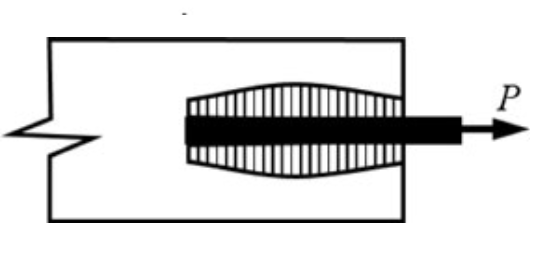
\includegraphics[width=0.3\columnwidth]{figs/Q16d.png}  

\end{enumerate}

\item In a two-dimensional stress analysis, the state of stress at a point $P$ is  
\begin{align}
[\sigma] =
\myvec{ \sigma_{xx} & \tau_{xy} \\ \tau_{xy} & \sigma_{yy} }
\end{align}
The necessary and sufficient condition for existence of the state of pure shear at the point $P$, is \hfill \brak{GATE \ CE \ 2020}

\begin{enumerate}

\item $\sigma_{xx}\sigma_{yy} - \tau_{xy}^{2} = 0$  
\item $\tau_{xy} = 0$  
\item $\sigma_{xx} + \sigma_{yy} = 0$  
\item $(\sigma_{xx} - \sigma_{yy})^{2} + 4\tau_{xy}^{2} = 0$  

\end{enumerate}

\item During the process of hydration of cement, due to increase in Dicalcium Silicate (C$_2$S) content in cement clinker, the heat of hydration \hfill \brak{GATE \ CE \ 2020}

\begin{enumerate}
\begin{multicols}{4}
\item increases  
\item decreases  
\item initially decreases and then increases  
\item does not change  
\end{multicols}
\end{enumerate}

\item The Los Angeles test for stone aggregates is used to examine \hfill \brak{GATE \ CE \ 2020}

\begin{enumerate}

\item abrasion resistance  
\item crushing strength  
\item soundness  
\item specific gravity  

\end{enumerate}

\item Which one of the following statements is NOT correct? \hfill \brak{GATE \ CE \ 2020}

\begin{enumerate}

\item A clay deposit with a liquidity index greater than unity is in a state of plastic consistency.  
\item The cohesion of normally consolidated clay is zero when triaxial test is conducted under consolidated undrained condition.  
\item The ultimate bearing capacity of a strip foundation supported on the surface of sandy soil increases in direct proportion to the width of footing.  
\item In case of a point load, Boussinesq's equation predicts higher value of vertical stress at a point directly beneath the load as compared to Westergaard's equation.  

\end{enumerate}

\item In a soil investigation work at a site, Standard Penetration Test \brak{SPT} was conducted at every 1.5 m interval up to 30 m depth. At 3 m depth, the observed number of hammer blows for three successive 150 mm penetrations were 8, 6 and 9, respectively. The SPT N -- value at 3 m depth, is \hfill \brak{GATE \ CE \ 2020}

\begin{enumerate}
\begin{multicols}{4}
\item $23$  
\item $17$  
\item $15$  
\item $14$  
\end{multicols}
\end{enumerate}

\item Velocity of flow is proportional to the first power of hydraulic gradient in Darcy' s law. This law is applicable to \hfill \brak{GATE \ CE \ 2020}

\begin{enumerate}

\item laminar flow in porous media
\item transitional flow in porous media
\item turbulent flow in porous media
\item laminar as well as turbulent flow in porous media

\end{enumerate}

\item A body floating in a liquid is in a stable state of equilibrium if its  \hfill \brak{GATE \ CE \ 2020}

\begin{enumerate}

\item metacentre lies above its centre of gravity
\item metacentre lies below its centre of gravity
\item metacentre coincides with its centre of gravity
\item centre of gravity is below its centre of buoyancy

\end{enumerate}

\item Uniform flow with velocity $U$ makes an angle $\theta$ with the $y$-axis. The velocity potential ($\phi$), is  \hfill \brak{GATE \ CE \ 2020}

\begin{figure}[H]
    \centering
    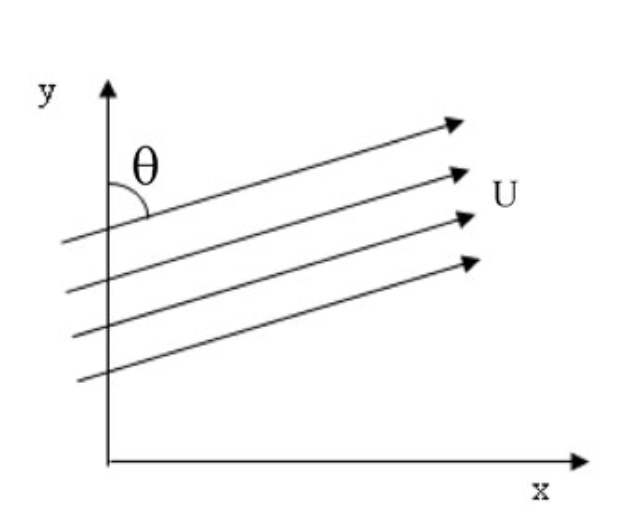
\includegraphics[width=0.3\columnwidth]{figs/Q24.png} 
    \caption{}
    \label{fig:placeholder}
\end{figure}

\begin{enumerate}

\item $\pm U (x \sin\theta + y \cos\theta)$\\
\item $\pm U (y \sin\theta - x \cos\theta)$\\
\item $\pm U (x \sin\theta - y \cos\theta)$\\
\item $\pm U (y \sin\theta + x \cos\theta)$

\end{enumerate}

\item The data for an agricultural field for a specific month are given below:  
Pan Evaporation = $100$ mm  
Effective Rainfall = $20$ mm  
Crop Coefficient = $0.4$  
Irrigation Efficiency = $0.5$  

The amount of irrigation water \brak{in \ mm} to be applied to the field in that month, is  \hfill \brak{GATE \ CE \ 2020}

\begin{enumerate}
\begin{multicols}{4}
\item 0
\item 20
\item 40
\item 80
\end{multicols}
\end{enumerate}

\item During chlorination process, aqueous (aq) chlorine reacts rapidly with water to form $\mathrm{Cl^-},\ \mathrm{HOCl}$ and $\mathrm{H^+}$ as shown below  
\begin{align}
\mathrm{Cl_2 (aq) + H_2O \rightleftharpoons HOCl + Cl^- + H^+}
\end{align}
The most active disinfectant in the chlorination process from amongst the following, is  \hfill \brak{GATE \ CE \ 2020}

\begin{enumerate}
\begin{multicols}{4}
\item $\mathrm{H^+}$
\item $\mathrm{HOCl}$
\item $\mathrm{Cl^-}$
\item $\mathrm{H_2O}$
\end{multicols}
\end{enumerate}

\item An amount of $35.67$ mg HCl is added to distilled water and the total solution volume is made to one litre. The atomic weights of H and Cl are 1 and 35.5, respectively. Neglecting the dissociation of water, the pH of the solution, is  \hfill \brak{GATE \ CE \ 2020}

\begin{enumerate}
\begin{multicols}{4}
\item $3.50$
\item $3.01$
\item $2.50$
\item $2.01$
\end{multicols}
\end{enumerate}

\item The probability that a 50 year flood may NOT occur at all during 25 years life of a project \emph{(round off to two decimal places)}, is \underline{\hspace{2cm}}.  \hfill \brak{GATE \ CE \ 2020}

\item A planar elastic structure is subjected to uniformly distributed load (not drawn to the scale). Neglecting self -- weight, the maximum bending moment generated in the structure (in kN.m, \emph{round off to the nearest integer}), is \underline{\hspace{2cm}}.  \hfill \brak{GATE \ CE \ 2020}

\begin{figure}[H]
    \centering
    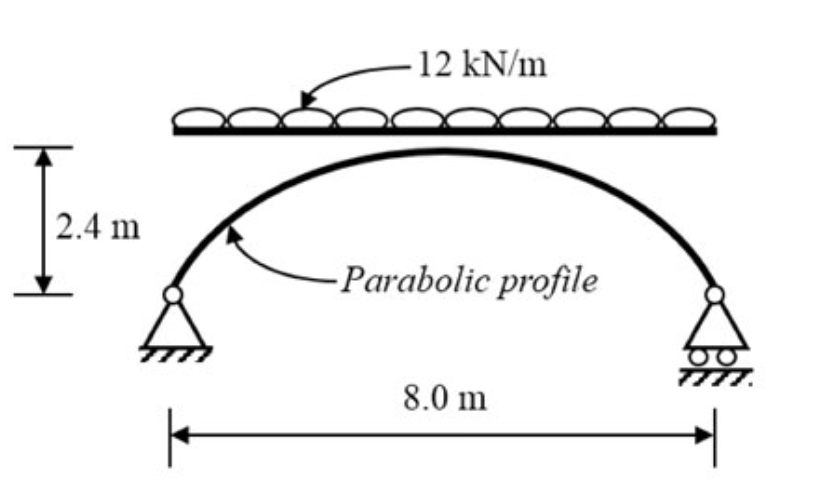
\includegraphics[width=0.3\columnwidth]{figs/Q29.png} 
    \caption{}
    \label{fig:placeholder}
\end{figure}

\item In an urban area, a median is provided to separate the opposing streams of traffic. As per IRC -- $86$ : $1983$, the desirable minimum width \brak{in \ m \ , expressed \ as \ integer} of the median, is \underline{\hspace{2cm}}.  \hfill \brak{GATE \ CE \ 2020}


\item A road in a hilly terrain is to be laid at a gradient of $4.5$ \%. A horizontal curve of radius $100$ m is laid at a location on this road. Gradient needs to be eased due to combination of curved horizontal and vertical profiles of the road. As per IRC, the compensated gradient (in \%, \emph{round off to one decimal place}), is \underline{\hspace{2cm}}. \hfill \brak{GATE \ CE \ 2020}

\item In a drained triaxial compression test, a sample of sand fails at deviator stress of 150 kPa under confining pressure of 50 kPa. The angle of internal friction (in degree, \emph{round off to the nearest integer}) of the sample, is \underline{\hspace{2cm}}.  \hfill \brak{GATE \ CE \ 2020}

\item A fully submerged infinite sandy slope has an inclination of $30^\degree$ with the horizontal. The saturated unit weight and effective angle of internal friction of sand are $18$ kN/m$^3$ and $38^\degree$, respectively. The unit weight of water is $10$ kN/m$^3$. Assume that the seepage is parallel to the slope. Against shear failure of the slope, the factor of safety (\emph{round off to two decimal places}) is \underline{\hspace{2cm}}.\hfill \brak{GATE \ CE \ 2020}

\item A $4$ m wide rectangular channel carries 6 m$^3$/s of water. The Manning's ' $n$'  of the open channel is 0.02. Considering $g=9.81$ m/s$^{2}$, the critical velocity of flow (in m/s, \brak{round off to two decimal places}) in the channel, is \underline{\hspace{2cm}}. \hfill \brak{GATE \ CE \ 2020}

\item A river has a flow of $1000$ million litres per day (MLD), BOD$_{5}$ of 5 mg/litre and Dissolved Oxygen (DO) level of $8$ mg/litre before receiving the wastewater discharge at a location. For the existing environmental conditions, the saturation DO level is 10 mg/litre in the river. Wastewater discharge of $100$ MLD with the BOD$_{5}$ of 200 mg/litre and DO level of $2$ mg/litre falls at that location. Assuming complete mixing of wastewater and river water, the immediate DO deficit (in mg/litre, \emph{round off to two decimal places}), is \underline{\hspace{2cm}}.  \hfill \brak{GATE \ CE \ 2020}

\noindent \textbf{Q36 -- Q65 carry two mark each.}

\item For the Ordinary Differential Equation
\begin{align}
\frac{d^{2}x}{dt^{2}} - 5 \frac{dx}{dt} + 6x = 0,
\end{align}
with initial conditions $x(0)=0$ and $\frac{dx}{dt}(0)=10$, the solution is \hfill \brak{GATE \ CE \ 2020}

\begin{enumerate}
\begin{multicols}{4}
\item $-5e^{2t}+6e^{3t}$
\item $5e^{2t}+6e^{3t}$
\item $-10e^{2t}+10e^{3t}$
\item $10e^{2t}+10e^{3t}$
\end{multicols}
\end{enumerate}

\item A continuous function $f(x)$ is defined. If the third derivative at $x_i$ is to be computed by using the fourth order central finite-divided-difference scheme (with step length = $h$), the correct formula is \hfill \brak{GATE \ CE \ 2020}

\begin{enumerate}

\item $\displaystyle f'''(x_i) = \frac{-f(x_{i+3}) + 8f(x_{i+2}) - 13f(x_{i+1}) + 13f(x_{i-1}) - 8f(x_{i-2}) + f(x_{i-3})}{8h^{3}}$\\
\item $\displaystyle f'''(x_i) = \frac{f(x_{i+3}) - 8f(x_{i+2}) - 13f(x_{i+1}) + 13f(x_{i-1}) + 8f(x_{i-2}) + f(x_{i-3})}{8h^{3}}$\\
\item $\displaystyle f'''(x_i) = \frac{-f(x_{i+3}) - 8f(x_{i+2}) + 13f(x_{i+1}) + 13f(x_{i-1}) + 8f(x_{i-2}) - f(x_{i-3})}{8h^{3}}$\\
\item $\displaystyle f'''(x_i) = \frac{f(x_{i+3}) - 8f(x_{i+2}) + 13f(x_{i+1}) - 13f(x_{i-1}) - 8f(x_{i-2}) + f(x_{i-3})}{8h^{3}}$

\end{enumerate}

\item Distributed load(s) of $50 \ kN/m$ may occupy any position(s) (either continuously or in patches) on the girder $PQRST$ as shown in the figure \textit{(not drawn to the scale)}.  

\begin{figure}[H]
    \centering
    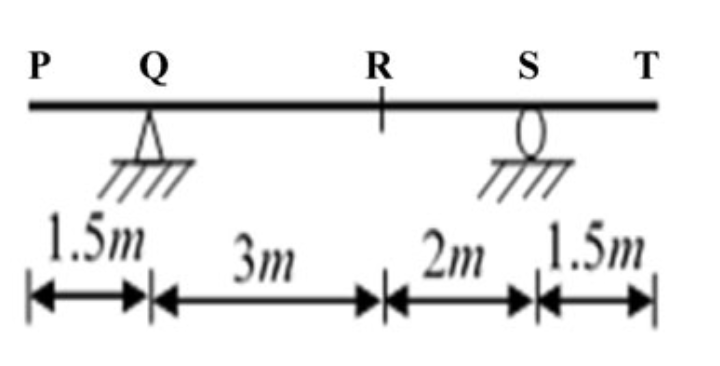
\includegraphics[width=0.3\columnwidth]{figs/Q38.png} 
    \caption{}
    \label{fig:placeholder}
\end{figure}

The maximum negative (hogging) bending moment \brak{in kN.m} that occurs at point $R$, is   \hfill \brak{GATE \ CE \ 2020}
\begin{enumerate}
\begin{multicols}{4}
\item $22.50$
\item $56.25$
\item $93.75$
\item $150.00$    
\end{multicols}

\end{enumerate}

\item A rigid weightless platform $PQRS$ shown in the figure \brak{not drawn to the scale} can slide freely in the vertical direction. The platform is held in position by the weightless member $OJ$ and four weightless, frictionless rollers. Points $O$ and $J$ are pin connections. A block of $90 \ kN$ rests on the platform as shown in the figure.  

\begin{figure}[H]
    \centering
    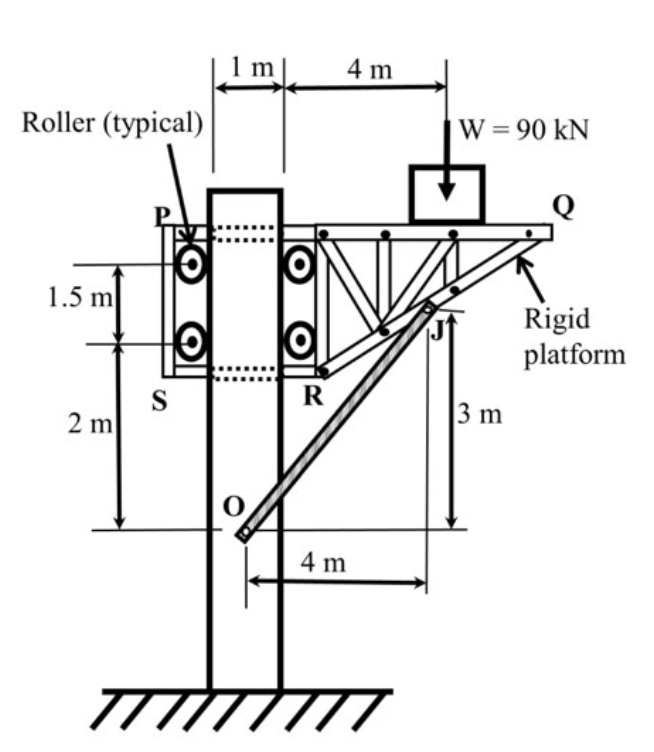
\includegraphics[width=0.3\columnwidth]{figs/Q39.png} 
    \caption{}
    \label{fig:placeholder}
\end{figure}

The magnitude of horizontal component of the reaction \brak{in \ kN} at pin $O$, is  \hfill \brak{GATE \ CE \ 2020}
\begin{enumerate}
\begin{multicols}{4}
\item $90$
\item $120$
\item $150$
\item $180$    
\end{multicols}

\end{enumerate}

\item A cantilever beam $PQ$ of uniform flexural rigidity $(EI)$ is subjected to a concentrated moment $M$ at $R$ as shown in the figure.  

\begin{figure}[H]
    \centering
    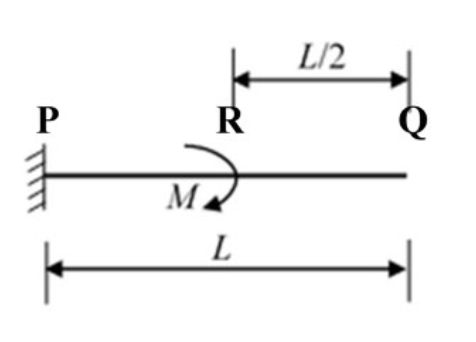
\includegraphics[width=0.3\columnwidth]{figs/Q40.png} 
    \caption{}
    \label{fig:placeholder}
\end{figure}

The deflection at the free end $Q$ is  \hfill \brak{GATE \ CE \ 2020}
\begin{enumerate}
\begin{multicols}{4}
\item $\frac{ML^2}{6EI}$
\item $\frac{ML^2}{4EI}$
\item $\frac{3ML^2}{8EI}$
\item $\frac{ML^2}{2EI}$
\end{multicols}

\end{enumerate}

\item A dowel bar is placed at a contraction joint. When contraction occurs, the concrete slab cracks at predetermined location(s). Identify the arrangement, which shows the correct placement of dowel bar and the place of occurrence of the contraction crack(s).  \hfill \brak{GATE \ CE \ 2020}


\begin{enumerate}
\item 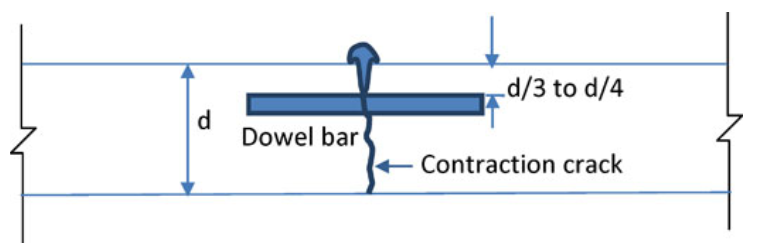
\includegraphics[width=0.3\columnwidth]{figs/Q41a.png}
\item 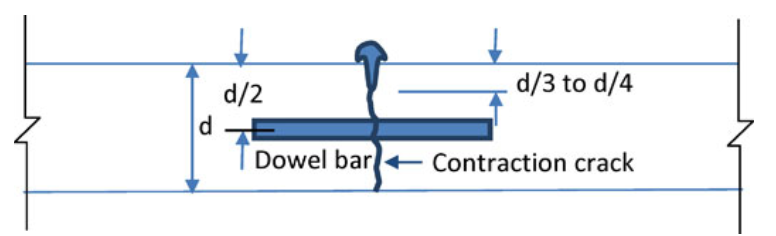
\includegraphics[width=0.3\columnwidth]{figs/Q41b.png}
\item 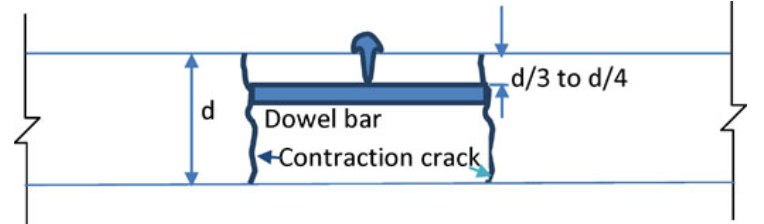
\includegraphics[width=0.3\columnwidth]{figs/Q41c.png}
\item 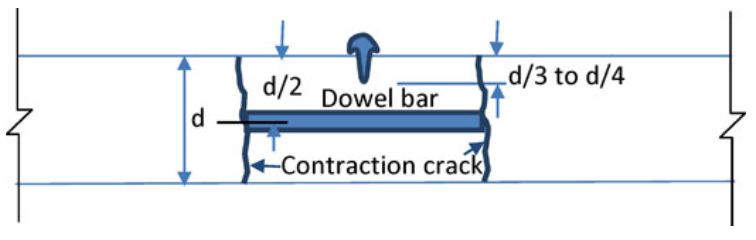
\includegraphics[width=0.3\columnwidth]{figs/Q41d.png}
\end{enumerate}


\item The relationship between traffic flow rate ($q$) and density ($D$) is shown in the figure.  

\begin{figure}[H]
    \centering
    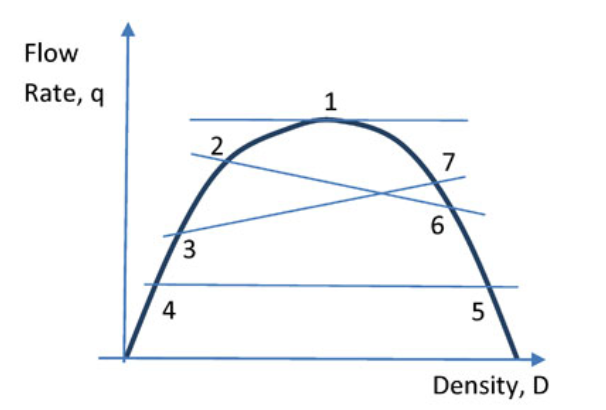
\includegraphics[width=0.3\columnwidth]{figs/Q42.png} 
    \caption{}
    \label{fig:placeholder}
\end{figure}

The shock wave condition is depicted by   \hfill \brak{GATE \ CE \ 2020}
\begin{enumerate}
\item flow with respect to point $1 \ (q_1 = q_2)$  
\item flow changing from point $2$ to point $6 \ (q_2 > q_6)$  
\item flow changing from point $3$ to point $7 \ (q_3 < q_7)$  
\item flow with respect to point $4$ and point $5 \ (q_4 = q_5)$  
\end{enumerate}

\item The appropriate design length of a clearway is calculated on the basis of Normal Take -- off condition. Which one of the following options correctly depicts the length of the clearway? \textit{(Note: None of the options are drawn to scale)}  
\hfill \brak{GATE \ CE \ 2020}
\begin{enumerate}
\item 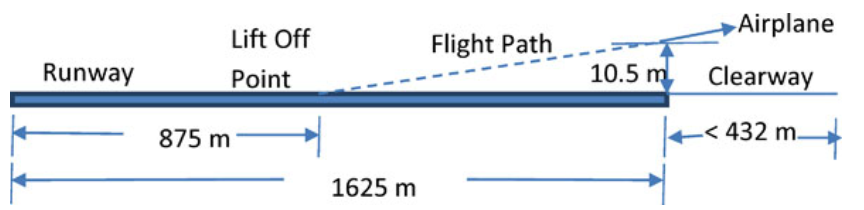
\includegraphics[width=0.3\columnwidth]{figs/Q43a.png}   
\item 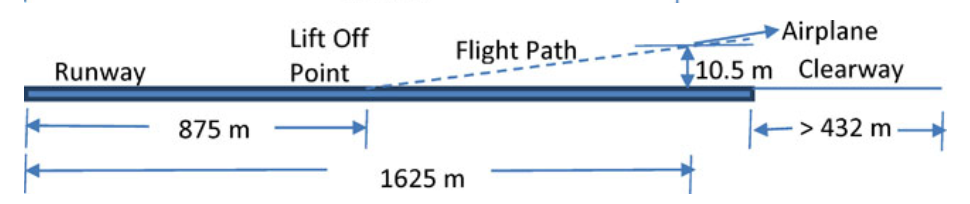
\includegraphics[width=0.3\columnwidth]{figs/Q43b.png}  
\item 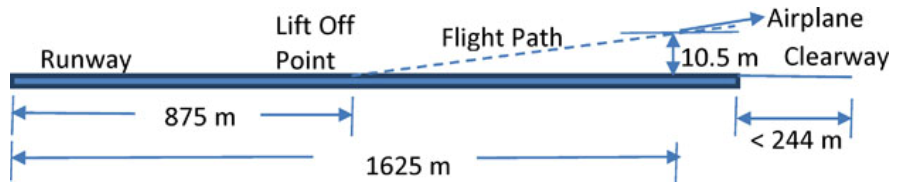
\includegraphics[width=0.3\columnwidth]{figs/Q43c.png}  
\item 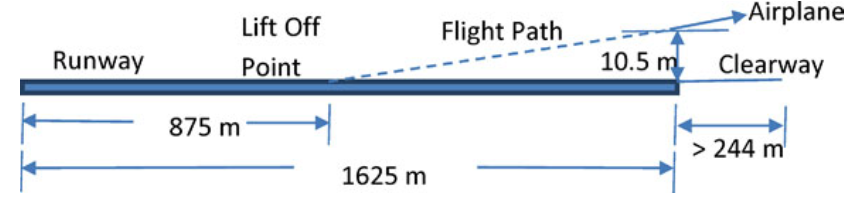
\includegraphics[width=0.3\columnwidth]{figs/Q43d.png}  
\end{enumerate}

\item The total stress paths corresponding to different loading conditions, for a soil specimen under the isotropically consolidated stress state $(O)$, are given.  

\begin{figure}[H]
    \centering
    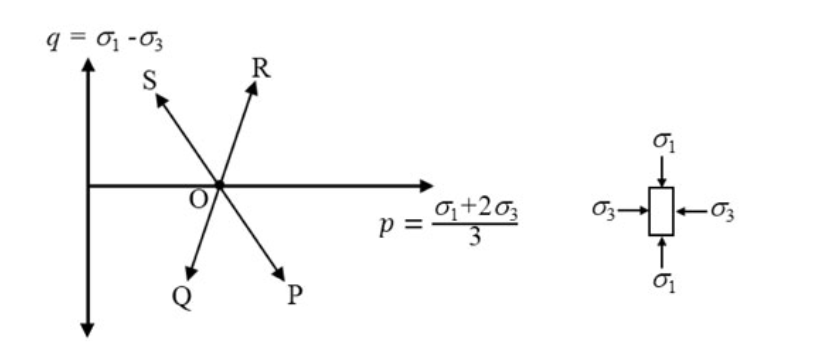
\includegraphics[width=0.3\columnwidth]{figs/Q44.png} 
    \caption{}
    \label{fig:placeholder}
\end{figure}

\begin{center}
\begin{tabular}{ll}
    \textbf{Group I} & \textbf{Group II} \\
    P. Ferrite & 1. Hexagonal Close Packed (HCP) \\
    Q. Austenite & 2. Body Centered Cubic (BCC) \\
    R. Martensite & 3. Body Centered Tetragonal (BCT) \\
    & 4. Face Centered Cubic (FCC)
\end{tabular}
\end{center}

The correct match between the stress paths and the listed loading conditions is  \hfill \brak{GATE \ CE \ 2020}
\begin{enumerate}
\item OP - I, OQ - II, OR - IV, OS - III  
\item OP - IV, OQ - III, OR - I, OS - II  
\item OP - III, OQ - II, OR - I, OS - IV  
\item OP - I, OQ - III, OR - II, OS - IV  
\end{enumerate}

\item The soil profile at a site up to a depth of $10 \ m$ is shown (not drawn to scale). The soil is preloaded with a uniform surcharge $(q)$ of $70 \ kN/m^2$ at the ground level. The water table is at a depth of $3 \ m$ below ground level. The soil unit weight of the respective layers is given. Consider unit weight of water as $9.81 \ kN/m^3$ and assume that the surcharge $(q)$ is applied instantaneously.  

\begin{figure}[H]
    \centering
    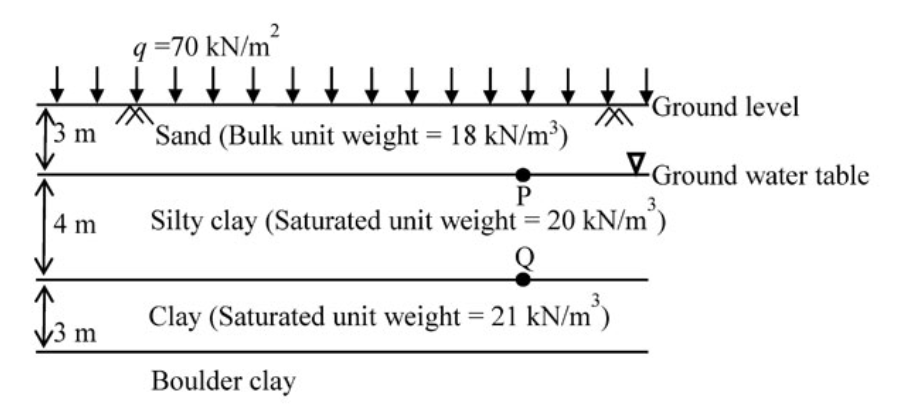
\includegraphics[width=0.3\columnwidth]{figs/Q45.png} 
    \caption{}
    \label{fig:placeholder}
\end{figure}

Immediately after preloading, the effective stresses \brak{in \ kPa} at points $P$ and $Q$, respectively, are:  \hfill \brak{GATE \ CE \ 2020}
\begin{enumerate}
\item $124$ and $204$  
\item $36$ and $90$  
\item $36$ and $126$  
\item $54$ and $95$  
\end{enumerate}

\item Water flows at the rate of $12 \ m^3/s$ in a $6 \ m$ wide rectangular channel. A hydraulic jump is formed in the channel at a point where the upstream depth is $30 \ cm$ (just before the jump). Considering acceleration due to gravity as $9.81 \ m/s^2$ and density of water as $1000 \ kg/m^3$, the energy loss in the jump is  \hfill \brak{GATE \ CE \ 2020}
\begin{enumerate}
\item $114.2 \ kW$  
\item $114.2 \ MW$  
\item $141.2 \ hp$  
\item $141.2 \ J/s$  
\end{enumerate}

\item A water supply scheme transports $10 \ MLD$ (Million Litres per Day) water through a $450 \ mm$ diameter pipeline for a distance of $2.5 \ km$. A chlorine dose of $3.50 \ mg/\text{litre}$ is applied at the starting point of the pipeline to attain a certain level of disinfection at the downstream end. It is decided to increase the flow rate from $10 \ MLD$ to $13 \ MLD$ in the pipeline. Assume exponent for concentration, $n = 0.86$. With this increased flow, in order to attain the same level of disinfection, the chlorine dose \brak{in \ mg/litre} to be applied at the starting point should be  \hfill \brak{GATE \ CE \ 2020}
\begin{enumerate}
\item $3.95$  
\item $4.40$  
\item $4.75$  
\item $5.55$  
\end{enumerate}

\item An open traverse $PQRST$ is surveyed using theodolite and the consecutive coordinates obtained are given in the table:  

\begin{tabular}{|c|c|c|}
     \hline
     \textbf{Mineral} & \textbf{Modal abundance \brak{\%}} & \textbf{Partition coefficient}\\
     \hline
     Clinopyroxene & $45$ & $0.506$ \\
      \hline
      Orthopyroxene & $40$ & $0.42$ \\
      \hline
      Olivine & $10$ & $0.045$ \\
      \hline
      Plagioclase & $05$ & $0.019$ \\
      \hline
\end{tabular}

If the independent coordinates (Northing, Easting) of station P are (400 m, 200 m), the independent coordinates \brak{in m} of station T are:  \hfill \brak{GATE \ CE \ 2020}
\begin{enumerate}
\item $194.7$, $370.1$  
\item $205.3$, $429.9$  
\item $394.7$, $170.1$  
\item $405.3$, $229.9$  
\end{enumerate}

\item If $C$ represents a line segment between $(0,0,0)$ and $(1,1,1)$ in Cartesian coordinate system, the value (expressed as integer) of the line integral  
\begin{align}
\int_C \left[ (y+z)dx + (x+z)dy + (x+y)dz \right]
\end{align}  
is \underline{\hspace{2cm}}. \hfill \brak{GATE \ CE \ 2020}

\item Consider the system of equations  

\myvec{ $1$ & $3$ & $2$ \\ $2$ & $2$ & $-3$ \\ $4$ & $4$ & $-6$ \\ $2$ & $5$ & $2$}
\myvec{x_1 \\ x_2 \\ x_3}
=
\myvec{$1$ \\$2$ \\$3$ \\$2$}

The value of $x_3$ \brak{round \ off \ to \ the \ nearest \ integer}, is \underline{\hspace{2cm}}. \hfill \brak{GATE \ CE \ 2020}

\item A rigid, uniform, weightless, horizontal bar is connected to three vertical members P, Q and R as shown (not drawn to scale). All three members have identical axial stiffness of $10 \ kN/mm$. The lower ends of bars P and R rest on a rigid horizontal surface. When no load is applied, a gap of $2 \ mm$ exists between the lower end of the bar Q and the rigid horizontal surface. When a vertical load $W$ is placed on the horizontal bar in the downward direction, the bar still remains horizontal and gets displaced by $5 \ mm$ in the vertically downward direction.  

\begin{figure}[H]
    \centering
    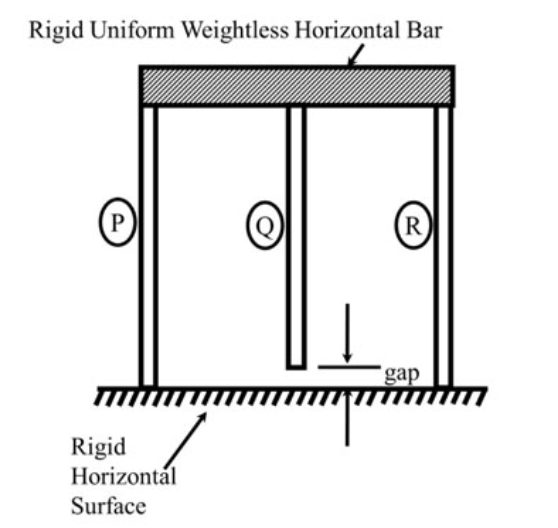
\includegraphics[width=0.3\columnwidth]{figs/Q51.png} 
    \caption{}
    \label{fig:placeholder}
\end{figure}

The magnitude of the load $W$ \brak{in \ kN \, round \ off \ to \ the \ nearest \ integer}, is \underline{\hspace{2cm}}. \hfill \brak{GATE \ CE \ 2020}

\item The flanges and web plates of the doubly symmetric built -- up section are connected by continuous $10 \ mm$ thick fillet welds as shown \brak{not \ drawn \ to \ scale}. The moment of inertia of the section about its principal axis X -- X is $7.73 \times 10^7 \ mm^4$. The permissible shear stress in the fillet welds is $100 \ N/mm^2$. The design shear strength of the section is governed by the capacity of the fillet welds.  

\begin{figure}[H]
    \centering
    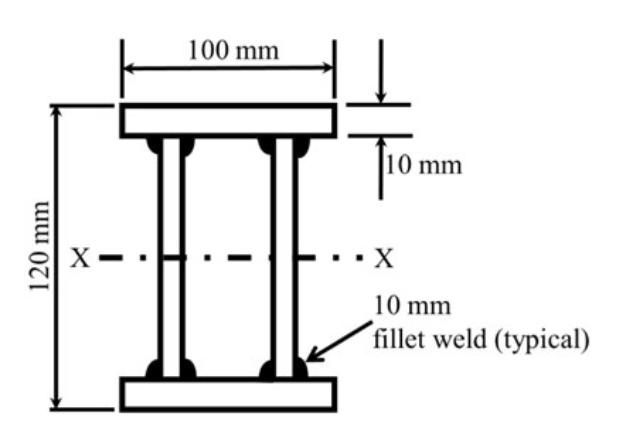
\includegraphics[width=0.3\columnwidth]{figs/Q52.png} 
    \caption{}
    \label{fig:placeholder}
\end{figure}

The maximum shear \brak{in \ kN, round \ off \ to \ one \ decimal \ place} that can be carried by the section is \underline{\hspace{2cm}}. \hfill \brak{GATE \ CE \ 2020}

\item A simply reinforced concrete beam section shown \brak{not \ drawn \ to \ scale} is made of M35 grade concrete and Fe600 grade reinforcing steel. The total cross-sectional area of the tension steel is $942 \ mm^2$.  

\begin{figure}[H]
    \centering
    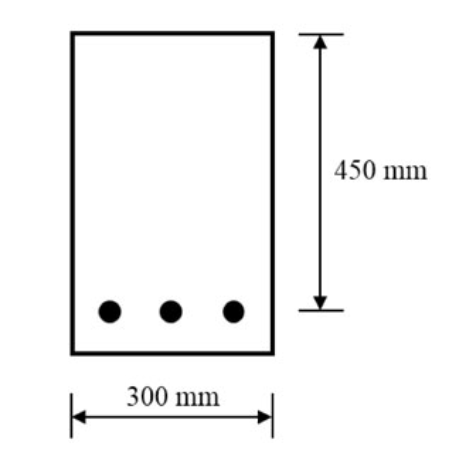
\includegraphics[width=0.3\columnwidth]{figs/Q53.png} 
    \caption{}
    \label{fig:placeholder}
\end{figure}

As per Limit State Design of IS $456$ : $2000$, the design moment capacity \brak{in \ kN.m, round \ off \ to \ two \ decimal \ places} of the beam section is \underline{\hspace{2cm}}. \hfill \brak{GATE \ CE \ 2020}

\item A simply supported prestressed concrete beam of rectangular cross-section, having a span of $9 \ m$, is prestressed with an effective prestressing force of $600 \ kN$. The eccentricity of the prestressing tendon at its two supports was linearly varied to a value of $e$ at the mid-span. In order to balance an external concentrated load of $12 \ kN$ applied at the mid-span, the required value of $e$ \brak{in \ mm, \ round \ off \ to \ the \ nearest \ integer} of the tendon, is \underline{\hspace{2cm}}. \hfill \brak{GATE \ CE \ 2020}

\item Traffic volume count has been collected on a 2 -- lane road section which needs upgradation due to severe traffic flow condition. Maximum service flow rate per lane is observed as $1720 \ veh/h$ at level of service 'C'. The Peak Hour Factor is reported as $0.72$. Historical traffic volume count provides Annual Average Daily Traffic as $12720 \ veh/day$. Differential split of the traffic flow is observed to be 60:40. Assuming that traffic stream consists of 'All Cars' and all drivers are 'Regular Commuters', the number of extra lane(s) \brak{round \ off \ to \ the \ next \ higher \ integer} to be provided is \underline{\hspace{2cm}}. \hfill \brak{GATE \ CE \ 2020}

\item A vertical retaining wall of $5 \ m$ height has to support soil having unit weight of $18 \ kN/m^3$, effective cohesion of $12 \ kN/m^2$ and effective friction angle of $30^\degree$. As per Rankine's earth pressure theory and assuming that a tension crack has occurred, the lateral active thrust on the wall per meter length (in kN, round off to two decimal places), is \underline{\hspace{2cm}}. \hfill \brak{GATE \ CE \ 2020}

\item Water flows in the upward direction in a tank through $2.5 \ m$ thick sand layer as shown. The void ratio and specific gravity of sand are $0.38$ and $2.7$, respectively. The sand is fully saturated. Unit weight of water is $10 \ kN/m^3$.  

\begin{figure}[H]
    \centering
    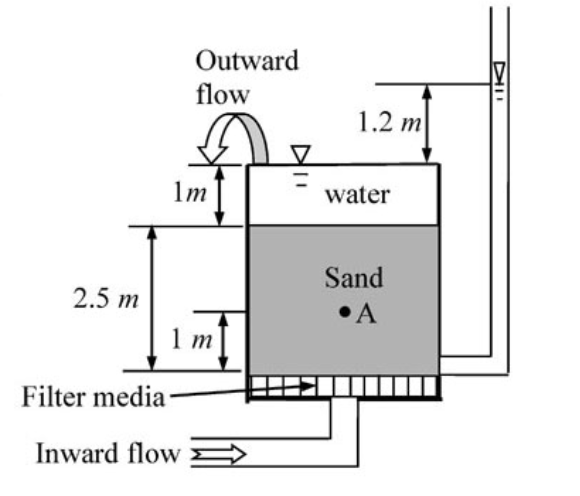
\includegraphics[width=0.3\columnwidth]{figs/Q57.png} 
    \caption{}
    \label{fig:placeholder}
\end{figure}

The effective stress \brak{in \ kPa, \ round \ off \ to \ two \ decimal \ places} at point A, located 1 m above the base of tank, is \underline{\hspace{2cm}}. \hfill \brak{GATE \ CE \ 2020}

\item A $10 \ m$ thick clay layer is resting over a $3 \ m$ thick sand layer and is submerged. A fill of $2 \ m$ thick sand with unit weight of $20 \ kN/m^3$ is placed above the clay layer to accelerate the rate of consolidation of the clay layer. Coefficient of consolidation of clay is $5 \times 10^{-2} \ m^2/year$ and coefficient of volume compressibility of clay is $2.2 \times 10^{-4} \ m^2/kN$. Assume Terzaghi's relation between time factor and average degree of consolidation.  


\begin{figure}[H]
    \centering
    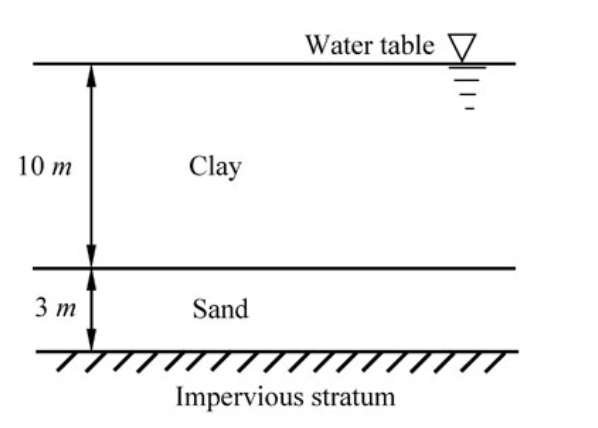
\includegraphics[width=0.3\columnwidth]{figs/Q58.png} 
    \caption{}
    \label{fig:placeholder}
\end{figure}

The settlement \brak{in \ mm, \ round \ off \ to \ two \ decimal \ places} of the clay layer, $10$ years after the construction of the fill, is \underline{\hspace{2cm}}. \hfill \brak{GATE \ CE \ 2020}


\item Three reservoirs P, Q, and R are interconnected by pipes as shown in the figure \textit{(not drawn to the scale)}. Piezometric head at the junction S of the pipes is $100 \ m$. Assume acceleration due to gravity as $9.81 \ m/s^2$ and density of water as $1000 \ kg/m^3$. The length of the pipe from junction S to the inlet of reservoir R is $180 \ m$. 

\begin{figure}[H]
    \centering
    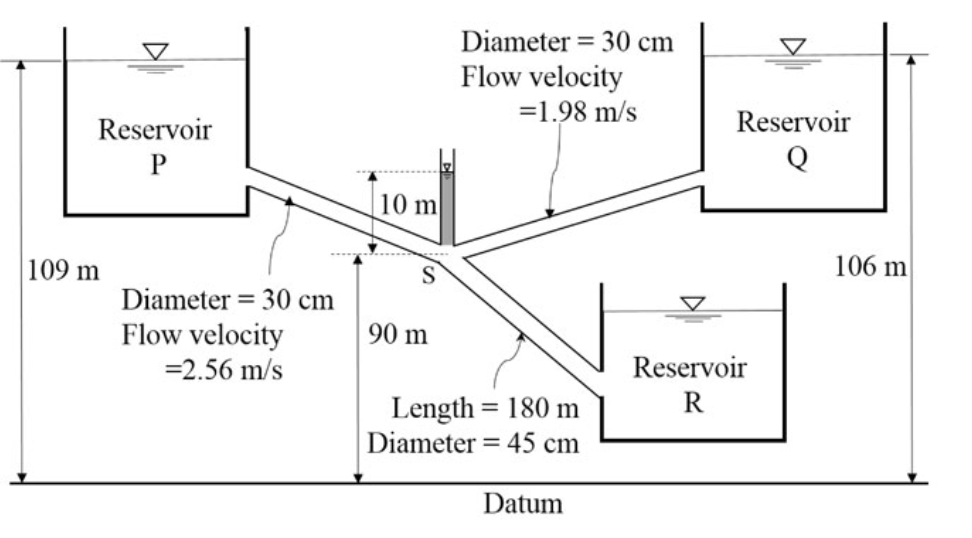
\includegraphics[width=0.3\columnwidth]{figs/Q59.png} 
    \caption{}
    \label{fig:placeholder}
\end{figure}

Considering head loss only due to friction (with friction factor of $0.03$ for all the pipes), the height of water level in the lowermost reservoir R \brak{in \ m, \ round \ off \ to \ one \ decimal \ place} with respect to the datum, is \_\_\_\_\_\_\_\_\_\_\_\_ . \hfill \brak{GATE \ CE \ 2020}

\item In a homogeneous unconfined aquifer of area $3.00 \ km^2$, the water table was at an elevation of $102.00 \ m$. After a natural recharge of volume $0.90$ million cubic meter (Mm$^3$), the water table rose to $103.20 \ m$. After this recharge, groundwater pumping took place and the water table dropped down to $101.20 \ m$. The volume of groundwater pumped after the natural recharge, expressed (in Mm$^3$ and \textit{round off to two decimal places}), is \_\_\_\_\_\_\_\_\_\_\_\_ . \hfill \brak{GATE \ CE \ 2020}
\item A circular water tank of $2 \ m$ diameter has a circular orifice of diameter $0.1 \ m$ at the bottom. Water enters the tank steadily at a flow rate of $20 \ litre/s$ and escapes through the orifice. The coefficient of discharge of the orifice is $0.8$. Consider the acceleration due to gravity as $9.81 \ m/s^2$ and neglect frictional losses. The height of the water level \brak{in \ m, \ round \ off \ to \ two \ decimal \ places} in the tank at the steady state, is \_\_\_\_\_\_\_\_\_\_\_\_ . \hfill \brak{GATE \ CE \ 2020}

\item Surface Overflow Rate \brak{SOR} of a primary settling tank (discrete settling) is $20000 \ litre/m^2$ per day. Kinematic viscosity of water in the tank is $1.01 \times 10^{-2} \ cm^2/s$. Specific gravity of the settling particles is $2.64$. Acceleration due to gravity is $9.81 \ m/s^2$. The minimum diameter (in $\mu m$, \textit{round off to one decimal place}) of the particles that will be removed with $80\%$ efficiency in the tank, is \_\_\_\_\_\_\_\_\_\_\_\_ . \hfill \brak{GATE \ CE \ 2020}

\item A gaseous chemical has a concentration of $41.6 \ \mu mol/m^3$ in air at $1 \ atm$ pressure and temperature $293 \ K$. The universal gas constant $R$ is $82.05 \times 10^{-6} \ (m^3 \ atm)/(mol \ K)$. Assuming that ideal gas law is valid, the concentration of the gaseous chemical \brak{in \ ppm, \ round \ off \ to \ one \ decimal \ place}, is \_\_\_\_\_\_\_\_\_\_\_\_ . \hfill \brak{GATE \ CE \ 2020}

\item A stream with a flow rate of $5 \ m^3/s$ is having an ultimate BOD of $30 \ mg/litre$. A wastewater discharge of $0.20 \ m^3/s$ having BOD$_5$ of $500 \ mg/litre$ joins the stream at a location and instantaneously gets mixed up completely. The cross-sectional area of the stream is $40 \ m^2$ which remains constant. BOD exertion rate constant is $0.3$ per day (logarithm base to $e$). The BOD (in $mg/litre$, \textit{round off to two decimal places}) remaining at $3 \ km$ downstream from the mixing location, is \_\_\_\_\_\_\_\_\_\_\_\_ . \hfill \brak{GATE \ CE \ 2020}

\item The lengths and bearings of a traverse PQRS are: 

\begin{table}[htbp]
  \centering
  \caption{Table-3}
  \label{table3}
  \begin{tabular}{cc}
  \textbf{Processing Technique} & \textbf{Producct} \\ \\
    P. Calendering & 1. Pipes \\
    Q. Extrusion & 2. Disposable cups \\
    R. Injection moulding & 3. Sheets \\
    S. Thermoforming & 4. Nylon gears \\
  \end{tabular}
\end{table}

The length of line segment SP (in m, \textit{round off to two decimal places}) is \_\_\_\_\_\_\_\_\_\_\_\_ . \hfill \brak{GATE \ CE \ 2020}


\end{enumerate}



\end{document}